\chapter{Evaluation}

\begin{figure}[hbtp]
	\centering
	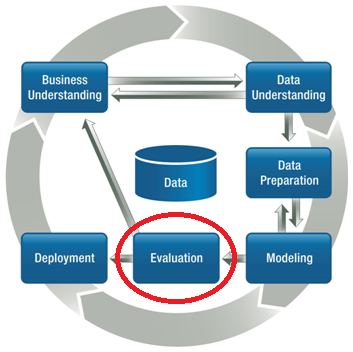
\includegraphics[width=0.5\textwidth]{./images/CRISPDM_5.png}
	\caption{CRISP-DM - Evaluation}
	\label{CRISPDM_5}
\end{figure}
In questa fase si andranno a valutare i risultati ottenuti dall'intero processo CRISP-DM fatto finora. Se tale valutazione risulta essere non positiva rispetto a ciò che il sistema si prefiggeva di fare, si passerà alla definizione di altri parametri o alla scelta di altri tipi di algoritmi per effettuare la classificazione.

\section{Valutazione rispetto agli obiettivi di business}
I risultati ottenuti, mostrati nella tabella \ref{tab:FTExtendFiltered}, possono essere considerati positivi rispetto agli obiettivi di business, in quanto supera il 99 \% di correttezza richiesto dal task \ref{task}. 
Tuttavia, al fine di tentare di migliorare ulteriormente il sistema di classificazione, sono state testate le varianti che il modello FT offriva (\emph{Alberi funzionali ai soli nodi intermedi} \ref{Alberi funzionali ai soli nodi intermedi} e \emph{Alberi funzionali ai soli nodi foglia} \ref{Alberi funzionali ai soli nodi foglia}). Per fare ciò, è stato necessario variare il parametro modelType rispettivamente in \emph{FT Inner} e \emph{FT Leaves}.

Inoltre, per completezza, è stato fatto un esperimento controllato avente n fattori con m livelli, in particolare 3 fattori:
%sono state sperimentate altre configurazioni sul dataset combinando tutti gli algoritmi definiti finora :
\textbf{Sampling} con 2 livelli:
\begin{itemize}
	\item Con SMOTE;
	\item Senza SMOTE;
\end{itemize}
\textbf{Feature Selection} con 2 livelli:
\begin{itemize}
	\item Con CfsSubsetEval;
	\item Senza CfsSubsetEval;
\end{itemize}
\textbf{Classifiers} con 3 livelli:
\begin{itemize}
	\item FT;
	\item FT-Leaves;
	\item FT-Inner.
\end{itemize}
\subsection{Risultati configurazioni}
Di seguito verranno riportati i risultati ottenuti da queste configurazioni: 
\paragraph{FT - Original Dataset}
{\footnotesize
	\begin{verbatim}
		=== Stratified cross-validation ===
		=== Summary ===
		
		Correctly Classified Instances        7910               98.875  %
		Incorrectly Classified Instances        90                1.125  %
		Kappa statistic                          0.9763
		Mean absolute error                      0.0139
		Root mean squared error                  0.1001
		Relative absolute error                  2.9227 %
		Root relative squared error             20.5236 %
		Total Number of Instances             8000     
		
		=== Detailed Accuracy By Class ===
		
		                TP Rate   FP Rate   Precision   Recall  F-Measure   ROC Area  Class
		                 0.984     0.008      0.987     0.984     0.986      0.994    yes
		                 0.992     0.016      0.99      0.992     0.991      0.994    no
		Weighted Avg.    0.989     0.013      0.989     0.989     0.989      0.994
		
		=== Confusion Matrix ===
		
		  a     b   <-- classified as
		3063   49 |      a = yes
		41   4847 |      b = no
	\end{verbatim}
}
\paragraph{FT - CfsSubsetEval}
{\footnotesize
	\begin{verbatim}
	=== Stratified cross-validation ===
	=== Summary ===
	
	Correctly Classified Instances        7898               98.725  %
	Incorrectly Classified Instances       102                1.275  %
	Kappa statistic                          0.9731
	Mean absolute error                      0.0164
	Root mean squared error                  0.1072
	Relative absolute error                  3.4493 %
	Root relative squared error             21.996  %
	Total Number of Instances             8000     
	
	=== Detailed Accuracy By Class ===
	
	                TP Rate   FP Rate   Precision   Recall  F-Measure   ROC Area  Class
	                 0.979     0.007      0.988     0.979     0.984      0.99     yes
	                 0.993     0.021      0.987     0.993     0.99       0.99     no
	Weighted Avg.    0.987     0.016      0.987     0.987     0.987      0.99 
	
	=== Confusion Matrix ===
	
	  a     b   <-- classified as
	3046   66   |    a = yes
	36     4852 |    b = no
	\end{verbatim}
}
\paragraph{FT - SMOTE}
{\footnotesize
	\begin{verbatim}
	=== Stratified cross-validation ===
	=== Summary ===
	
	Correctly Classified Instances       10992               98.9201 %
	Incorrectly Classified Instances       120                1.0799 %
	Kappa statistic                          0.9781
	Mean absolute error                      0.0121
	Root mean squared error                  0.0972
	Relative absolute error                  2.4639 %
	Root relative squared error             19.5852 %
	Total Number of Instances            11112     
	
	=== Detailed Accuracy By Class ===
	
	                TP Rate   FP Rate   Precision   Recall  F-Measure   ROC Area  Class
	                 0.99      0.012      0.99      0.99      0.99       0.995    yes
	                 0.988     0.01       0.988     0.988     0.988      0.995    no
	Weighted Avg.    0.989     0.011      0.989     0.989     0.989      0.995
	
	=== Confusion Matrix ===
	
	  a     b   <-- classified as
	6164   60 |    a = yes
	60   4828 |    b = no
	\end{verbatim}
}
\paragraph{FT Inner - Original}
{\footnotesize
	\begin{verbatim}
	=== Stratified cross-validation ===
	=== Summary ===
	
	Correctly Classified Instances        7908               98.85   %
	Incorrectly Classified Instances        92                1.15   %
	Kappa statistic                          0.9758
	Mean absolute error                      0.0115
	Root mean squared error                  0.1072
	Relative absolute error                  2.4192 %
	Root relative squared error             21.9965 %
	Total Number of Instances             8000     
	
	=== Detailed Accuracy By Class ===
	
	                TP Rate   FP Rate   Precision   Recall  F-Measure   ROC Area  Class
	                 0.985     0.009      0.986     0.985     0.985      0.988    yes
	                 0.991     0.015      0.99      0.991     0.991      0.988    no
	Weighted Avg.    0.989     0.013      0.988     0.989     0.988      0.988
	
	=== Confusion Matrix ===
	
	 a      b   <-- classified as
	3064   48   |      a = yes
	44     4844 |      b = no
	
	\end{verbatim}
}
\paragraph{FT Inner - CfsSubsetEval}
{\footnotesize
	\begin{verbatim}
	=== Stratified cross-validation ===
	=== Summary ===
	
	Correctly Classified Instances        7896               98.7    %
	Incorrectly Classified Instances       104                1.3    %
	Kappa statistic                          0.9726
	Mean absolute error                      0.013 
	Root mean squared error                  0.114 
	Relative absolute error                  2.7347 %
	Root relative squared error             23.3871 %
	Total Number of Instances             8000     
	
	=== Detailed Accuracy By Class ===
	
	                TP Rate   FP Rate   Precision   Recall  F-Measure   ROC Area  Class
	                 0.978     0.007      0.988     0.978     0.983      0.985    yes
	                 0.993     0.022      0.986     0.993     0.989      0.985    no
	Weighted Avg.    0.987     0.016      0.987     0.987     0.987      0.985
	
	=== Confusion Matrix ===
	
	  a     b   <-- classified as
	3044   68   |    a = yes
	36     4852 |    b = no	
	\end{verbatim}
}
\paragraph{FT Inner - SMOTE}
{\footnotesize
	\begin{verbatim}
	=== Stratified cross-validation ===
	=== Summary ===
	
	Correctly Classified Instances       10985               98.8571 %
	Incorrectly Classified Instances       127                1.1429 %
	Kappa statistic                          0.9768
	Mean absolute error                      0.0114
	Root mean squared error                  0.1069
	Relative absolute error                  2.3193 %
	Root relative squared error             21.5376 %
	Total Number of Instances            11112     
	
	=== Detailed Accuracy By Class ===
	
	                TP Rate   FP Rate   Precision   Recall  F-Measure   ROC Area  Class
	                 0.991     0.014      0.989     0.991     0.99       0.988    yes
	                 0.986     0.009      0.988     0.986     0.987      0.988    no
	Weighted Avg.    0.989     0.012      0.989     0.989     0.989      0.988
	
	=== Confusion Matrix ===
	
	  a     b   <-- classified as
	6165   59   |    a = yes
	68     4820 |    b = no	
	\end{verbatim}
}
\paragraph{FT Inner - SMOTE - CfsSubsetEval}
{\footnotesize
	\begin{verbatim}
	=== Stratified cross-validation ===
	=== Summary ===
	
	Correctly Classified Instances       11001               99.0011 %
	Incorrectly Classified Instances       111                0.9989 %
	Kappa statistic                          0.9797
	Mean absolute error                      0.01  
	Root mean squared error                  0.0999
	Relative absolute error                  2.0271 %
	Root relative squared error             20.1353 %
	Total Number of Instances            11112     
	
	=== Detailed Accuracy By Class ===
	
	                TP Rate   FP Rate   Precision   Recall  F-Measure   ROC Area  Class
	                 0.988     0.008      0.994     0.988     0.991      0.99     yes
	                 0.992     0.012      0.985     0.992     0.989      0.99     no
	Weighted Avg.    0.99      0.009      0.99      0.99      0.99       0.99 
	
	=== Confusion Matrix ===
	
	  a     b   <-- classified as
	6150   74   |    a = yes
	37     4851 |    b = no
	\end{verbatim}
}
\paragraph{FT Leaves - Original}
{\footnotesize
	\begin{verbatim}
	=== Stratified cross-validation ===
	=== Summary ===
	
	Correctly Classified Instances        7926               99.075  %
	Incorrectly Classified Instances        74                0.925  %
	Kappa statistic                          0.9805
	Mean absolute error                      0.0139
	Root mean squared error                  0.0913
	Relative absolute error                  2.9172 %
	Root relative squared error             18.7372 %
	Total Number of Instances             8000     
	
	=== Detailed Accuracy By Class ===
	
	                TP Rate   FP Rate   Precision   Recall  F-Measure   ROC Area  Class
	                 0.985     0.005      0.992     0.985     0.988      0.998    yes
	                 0.995     0.015      0.99      0.995     0.992      0.998    no
	Weighted Avg.    0.991     0.011      0.991     0.991     0.991      0.998
	
	=== Confusion Matrix ===
	
	  a     b   <-- classified as
	3064   48   |    a = yes
	26     4862 |    b = no
	
	\end{verbatim}
}
\paragraph{FT Leaves - CfsSubsetEval}
{\footnotesize
	\begin{verbatim}
	=== Stratified cross-validation ===
	=== Summary ===
	
	Correctly Classified Instances        7901               98.7625 %
	Incorrectly Classified Instances        99                1.2375 %
	Kappa statistic                          0.9739
	Mean absolute error                      0.0214
	Root mean squared error                  0.1027
	Relative absolute error                  4.4989 %
	Root relative squared error             21.0674 %
	Total Number of Instances             8000     
	
	=== Detailed Accuracy By Class ===
	
	                TP Rate   FP Rate   Precision   Recall  F-Measure   ROC Area  Class
	                 0.978     0.006      0.99      0.978     0.984      0.997    yes
	                 0.994     0.022      0.986     0.994     0.99       0.997    no
	Weighted Avg.    0.988     0.016      0.988     0.988     0.988      0.997
	
	=== Confusion Matrix ===
	
	  a     b   <-- classified as
	3044   68   |    a = yes
	31     4857 |    b = no
	
	\end{verbatim}
}
\paragraph{FT Leaves - SMOTE}
{\footnotesize
	\begin{verbatim}
	=== Stratified cross-validation ===
	=== Summary ===
	
	Correctly Classified Instances       11028               99.2441 %
	Incorrectly Classified Instances        84                0.7559 %
	Kappa statistic                          0.9847
	Mean absolute error                      0.0121
	Root mean squared error                  0.0798
	Relative absolute error                  2.4485 %
	Root relative squared error             16.0749 %
	Total Number of Instances            11112     
	
	=== Detailed Accuracy By Class ===
	
	                TP Rate   FP Rate   Precision   Recall  F-Measure   ROC Area  Class
	                 0.991     0.005      0.996     0.991     0.993      0.997    yes
	                 0.995     0.009      0.988     0.995     0.991      0.997    no
	Weighted Avg.    0.992     0.007      0.992     0.992     0.992      0.997
	
	=== Confusion Matrix ===
	
	  a     b   <-- classified as
	6166   58   |    a = yes
	26     4862 |    b = no
	\end{verbatim}
}
\paragraph{FT Leaves - SMOTE - CfsSubsetEval}
{\footnotesize
	\begin{verbatim}
	=== Stratified cross-validation ===
	=== Summary ===
	
	Correctly Classified Instances       11009               99.0731 %
	Incorrectly Classified Instances       103                0.9269 %
	Kappa statistic                          0.9812
	Mean absolute error                      0.0175
	Root mean squared error                  0.0911
	Relative absolute error                  3.5547 %
	Root relative squared error             18.3503 %
	Total Number of Instances            11112     
	
	=== Detailed Accuracy By Class ===
	
	                TP Rate   FP Rate   Precision   Recall  F-Measure   ROC Area  Class
	                 0.988     0.006      0.995     0.988     0.992      0.997    yes
	                 0.994     0.012      0.985     0.994     0.99       0.997    no
	Weighted Avg.    0.991     0.009      0.991     0.991     0.991      0.997
	
	=== Confusion Matrix ===
	
	  a     b   <-- classified as
	6149   75   |    a = yes
	28     4860 |    b = no	
	\end{verbatim}
}

%
%\begin{table}[htbp]
%	\centering
%	\resizebox{1\textwidth}{!}{%
%		% Table generated by Excel2LaTeX from sheet 'FT Leaves'
%			\begin{tabular}{rrrrrrrrr}
%				\multicolumn{4}{c}{=== Stratified cross-validation ===} &       &       &       &       &  \\
%				\multicolumn{3}{c}{=== Summary ===} &       &       &       &       &       &  \\
%				&       &       &       &       &       &       &       &  \\
%				Correctly Classified Instances    & 11009 & \textit{\textbf{99,0731\%}} &       & \multicolumn{4}{c}{=== Confusion Matrix ===} & \multicolumn{1}{c}{} \\
%				Incorrectly Classified Instances & 103   & 0,9269\% &       &       &       &       &       &  \\
%				Kappa statistic   & 0,9812 &       &       & \multicolumn{1}{c}{\textit{\textbf{Yes}}} & \multicolumn{1}{c}{\textit{\textbf{No}}} & \multicolumn{1}{c}{<--} & \multicolumn{2}{c}{Classified as} \\
%				Mean absolute error & 0,0175 &       &       & \multicolumn{1}{c}{6149} & \multicolumn{1}{c}{75} &       &       &  \\
%				Root mean squared error & 0,0911 &       &       & \multicolumn{1}{c}{28} & \multicolumn{1}{c}{4860} &       &       &  \\
%				Relative absolute error & 3,55\% &       &       &       &       &       &       &  \\
%				Root relative squared error & 18,3503\% &       &       &       &       &       &       &  \\
%				Total Number of Instances      & 11112 &       &       &       &       &       &       &  \\
%				Attributes & 53    &       &       &       &       &       &       &  \\
%				\multicolumn{8}{c}{=== Detailed Accuracy By Class ===}        &  \\
%				&       &       &       &       &       &       &       &  \\
%				\multicolumn{1}{c}{} & \multicolumn{1}{c}{\textit{\textbf{TP Rate}}} & \multicolumn{1}{c}{\textit{\textbf{FP Rate}}} & \multicolumn{1}{c}{\textit{\textbf{Precision}}} & \multicolumn{1}{c}{\textit{\textbf{Recall}}} & \multicolumn{1}{c}{\textit{\textbf{F-Measure}}} & \multicolumn{1}{c}{\textit{\textbf{ROC Area}}} & \multicolumn{1}{c}{\textit{\textbf{Class}}} &  \\
%				\multicolumn{1}{c}{} & \multicolumn{1}{c}{0,988} & \multicolumn{1}{c}{0,006} & \multicolumn{1}{c}{0,995} & \multicolumn{1}{c}{0,988} & \multicolumn{1}{c}{0,992} & \multicolumn{1}{c}{0,997} & \multicolumn{1}{c}{yes} &  \\
%				\multicolumn{1}{c}{} & \multicolumn{1}{c}{0,994} & \multicolumn{1}{c}{0,012} & \multicolumn{1}{c}{0,985} & \multicolumn{1}{c}{0,994} & \multicolumn{1}{c}{0,99} & \multicolumn{1}{c}{0,997} & \multicolumn{1}{c}{no} &  \\
%				\multicolumn{1}{c}{} & \multicolumn{1}{c}{} & \multicolumn{1}{c}{} & \multicolumn{1}{c}{} & \multicolumn{1}{c}{} & \multicolumn{1}{c}{} & \multicolumn{1}{c}{} & \multicolumn{1}{c}{} &  \\
%				\multicolumn{1}{c}{\textit{\textbf{Weighted Avg.}}} & \multicolumn{1}{c}{0,991} & \multicolumn{1}{c}{0,009} & \multicolumn{1}{c}{0,991} & \multicolumn{1}{c}{0,991} & \multicolumn{1}{c}{0,991} & \multicolumn{1}{c}{0,997} & \multicolumn{1}{c}{} &  \\
%			\end{tabular}%
%	}
%	\label{tab:FTLeavesExtendFiltered}%
%	\caption{ SMOTE - CFSubsetEval - FT-Leaves}
%\end{table}%
%
%\begin{table}[htbp]
%	\centering
%	\resizebox{1\textwidth}{!}{%
%		% Table generated by Excel2LaTeX from sheet 'FT Inner'
%			\begin{tabular}{rrrrrrrrr}
%				\multicolumn{4}{c}{=== Stratified cross-validation ===} &       &       &       &       &  \\
%				\multicolumn{3}{c}{=== Summary ===} &       &       &       &       &       &  \\
%				&       &       &       &       &       &       &       &  \\
%				Correctly Classified Instances    & 11001 & \textit{\textbf{99,0011\%}} &       & \multicolumn{4}{c}{=== Confusion Matrix ===} & \multicolumn{1}{c}{} \\
%				Incorrectly Classified Instances & 111   & 0,9989\% &       &       &       &       &       &  \\
%				Kappa statistic   & 0,9797 &       &       & \multicolumn{1}{c}{\textit{\textbf{Yes}}} & \multicolumn{1}{c}{\textit{\textbf{No}}} & \multicolumn{1}{c}{<--} & \multicolumn{2}{c}{Classified as} \\
%				Mean absolute error & 0,01  &       &       & \multicolumn{1}{c}{6150} & \multicolumn{1}{c}{74} &       &       &  \\
%				Root mean squared error & 0,0999 &       &       & \multicolumn{1}{c}{37} & \multicolumn{1}{c}{4851} &       &       &  \\
%				Relative absolute error & 2,03\% &       &       &       &       &       &       &  \\
%				Root relative squared error & 20,1353\% &       &       &       &       &       &       &  \\
%				Total Number of Instances      & 11112 &       &       &       &       &       &       &  \\
%				Attributes & 53    &       &       &       &       &       &       &  \\
%				\multicolumn{8}{c}{=== Detailed Accuracy By Class ===}        &  \\
%				&       &       &       &       &       &       &       &  \\
%				\multicolumn{1}{c}{} & \multicolumn{1}{c}{\textit{\textbf{TP Rate}}} & \multicolumn{1}{c}{\textit{\textbf{FP Rate}}} & \multicolumn{1}{c}{\textit{\textbf{Precision}}} & \multicolumn{1}{c}{\textit{\textbf{Recall}}} & \multicolumn{1}{c}{\textit{\textbf{F-Measure}}} & \multicolumn{1}{c}{\textit{\textbf{ROC Area}}} & \multicolumn{1}{c}{\textit{\textbf{Class}}} &  \\
%				\multicolumn{1}{c}{} & \multicolumn{1}{c}{0,988} & \multicolumn{1}{c}{0,008} & \multicolumn{1}{c}{0,994} & \multicolumn{1}{c}{0,988} & \multicolumn{1}{c}{0,991} & \multicolumn{1}{c}{0,99} & \multicolumn{1}{c}{yes} &  \\
%				\multicolumn{1}{c}{} & \multicolumn{1}{c}{0,992} & \multicolumn{1}{c}{0,012} & \multicolumn{1}{c}{0,985} & \multicolumn{1}{c}{0,992} & \multicolumn{1}{c}{0,989} & \multicolumn{1}{c}{0,99} & \multicolumn{1}{c}{no} &  \\
%				\multicolumn{1}{c}{} & \multicolumn{1}{c}{} & \multicolumn{1}{c}{} & \multicolumn{1}{c}{} & \multicolumn{1}{c}{} & \multicolumn{1}{c}{} & \multicolumn{1}{c}{} & \multicolumn{1}{c}{} &  \\
%				\multicolumn{1}{c}{\textit{\textbf{Weighted Avg.}}} & \multicolumn{1}{c}{0,99} & \multicolumn{1}{c}{0,009} & \multicolumn{1}{c}{0,99} & \multicolumn{1}{c}{0,99} & \multicolumn{1}{c}{0,99} & \multicolumn{1}{c}{0,99} & \multicolumn{1}{c}{} &  \\
%			\end{tabular}%
%	}
%	\label{tab:FTInnerExtendFiltered}%
%	\caption{ SMOTE - CFSubsetEval - FT-Inner}
%\end{table}%
%
%\begin{table}[htbp]
%	\centering
%	\resizebox{1\textwidth}{!}{%
%		% Table generated by Excel2LaTeX from sheet 'FT'
%			\begin{tabular}{rrrrrrrrr}
%				\multicolumn{4}{c}{=== Stratified cross-validation ===} &       &       &       &       &  \\
%				\multicolumn{3}{c}{=== Summary ===} &       &       &       &       &       &  \\
%				&       &       &       &       &       &       &       &  \\
%				Correctly Classified Instances    & 10992 & \textit{\textbf{98,9201\%}} &       & \multicolumn{4}{c}{=== Confusion Matrix ===} & \multicolumn{1}{c}{} \\
%				Incorrectly Classified Instances & 120   & 1,0799\% &       &       &       &       &       &  \\
%				Kappa statistic   & 0,9781 &       &       & \multicolumn{1}{c}{\textit{\textbf{Yes}}} & \multicolumn{1}{c}{\textit{\textbf{No}}} & \multicolumn{1}{c}{<--} & \multicolumn{2}{c}{Classified as} \\
%				Mean absolute error & 0,0121 &       &       & \multicolumn{1}{c}{6164} & \multicolumn{1}{c}{60} &       &       &  \\
%				Root mean squared error & 0,0972 &       &       & \multicolumn{1}{c}{60} & \multicolumn{1}{c}{4828} &       &       &  \\
%				Relative absolute error & 2,46\% &       &       &       &       &       &       &  \\
%				Root relative squared error & 19,5852\% &       &       &       &       &       &       &  \\
%				Total Number of Instances      & 11112 &       &       &       &       &       &       &  \\
%				Attributes & 834   &       &       &       &       &       &       &  \\
%				\multicolumn{8}{c}{=== Detailed Accuracy By Class ===}        &  \\
%				&       &       &       &       &       &       &       &  \\
%				\multicolumn{1}{c}{} & \multicolumn{1}{c}{\textit{\textbf{TP Rate}}} & \multicolumn{1}{c}{\textit{\textbf{FP Rate}}} & \multicolumn{1}{c}{\textit{\textbf{Precision}}} & \multicolumn{1}{c}{\textit{\textbf{Recall}}} & \multicolumn{1}{c}{\textit{\textbf{F-Measure}}} & \multicolumn{1}{c}{\textit{\textbf{ROC Area}}} & \multicolumn{1}{c}{\textit{\textbf{Class}}} &  \\
%				\multicolumn{1}{c}{} & \multicolumn{1}{c}{0,99} & \multicolumn{1}{c}{0,012} & \multicolumn{1}{c}{0,99} & \multicolumn{1}{c}{0,99} & \multicolumn{1}{c}{0,99} & \multicolumn{1}{c}{0,995} & \multicolumn{1}{c}{yes} &  \\
%				\multicolumn{1}{c}{} & \multicolumn{1}{c}{0,988} & \multicolumn{1}{c}{0,01} & \multicolumn{1}{c}{0,988} & \multicolumn{1}{c}{0,988} & \multicolumn{1}{c}{0,988} & \multicolumn{1}{c}{0,995} & \multicolumn{1}{c}{no} &  \\
%				\multicolumn{1}{c}{} & \multicolumn{1}{c}{} & \multicolumn{1}{c}{} & \multicolumn{1}{c}{} & \multicolumn{1}{c}{} & \multicolumn{1}{c}{} & \multicolumn{1}{c}{} & \multicolumn{1}{c}{} &  \\
%				\multicolumn{1}{c}{\textit{\textbf{Weighted Avg.}}} & \multicolumn{1}{c}{0,989} & \multicolumn{1}{c}{0,011} & \multicolumn{1}{c}{0,989} & \multicolumn{1}{c}{0,989} & \multicolumn{1}{c}{0,989} & \multicolumn{1}{c}{0,995} & \multicolumn{1}{c}{} &  \\
%			\end{tabular}%
%	}
%	\label{tab:FTExtend}%
%	\caption{ SMOTE - Senza CFSubsetEval - FT}
%\end{table}%
%
%\begin{table}[htbp]
%	\centering
%	\resizebox{1\textwidth}{!}{%
%		% Table generated by Excel2LaTeX from sheet 'FT Leaves'
%			\begin{tabular}{rrrrrrrrr}
%				\multicolumn{4}{c}{=== Stratified cross-validation ===} &       &       &       &       &  \\
%				\multicolumn{3}{c}{=== Summary ===} &       &       &       &       &       &  \\
%				&       &       &       &       &       &       &       &  \\
%				Correctly Classified Instances    & 11028 & \textit{\textbf{99,2441\%}} &       & \multicolumn{4}{c}{=== Confusion Matrix ===} & \multicolumn{1}{c}{} \\
%				Incorrectly Classified Instances & 84    & 0,7559\% &       &       &       &       &       &  \\
%				Kappa statistic   & 0,9847 &       &       & \multicolumn{1}{c}{\textit{\textbf{Yes}}} & \multicolumn{1}{c}{\textit{\textbf{No}}} & \multicolumn{1}{c}{<--} & \multicolumn{2}{c}{Classified as} \\
%				Mean absolute error & 0,0121 &       &       & \multicolumn{1}{c}{6166} & \multicolumn{1}{c}{58} &       &       &  \\
%				Root mean squared error & 0,0798 &       &       & \multicolumn{1}{c}{26} & \multicolumn{1}{c}{4862} &       &       &  \\
%				Relative absolute error & 2,45\% &       &       &       &       &       &       &  \\
%				Root relative squared error & 16,0749\% &       &       &       &       &       &       &  \\
%				Total Number of Instances      & 11112 &       &       &       &       &       &       &  \\
%				Attributes & 834   &       &       &       &       &       &       &  \\
%				\multicolumn{8}{c}{=== Detailed Accuracy By Class ===}        &  \\
%				&       &       &       &       &       &       &       &  \\
%				\multicolumn{1}{c}{} & \multicolumn{1}{c}{\textit{\textbf{TP Rate}}} & \multicolumn{1}{c}{\textit{\textbf{FP Rate}}} & \multicolumn{1}{c}{\textit{\textbf{Precision}}} & \multicolumn{1}{c}{\textit{\textbf{Recall}}} & \multicolumn{1}{c}{\textit{\textbf{F-Measure}}} & \multicolumn{1}{c}{\textit{\textbf{ROC Area}}} & \multicolumn{1}{c}{\textit{\textbf{Class}}} &  \\
%				\multicolumn{1}{c}{} & \multicolumn{1}{c}{0,991} & \multicolumn{1}{c}{0,005} & \multicolumn{1}{c}{0,996} & \multicolumn{1}{c}{0,991} & \multicolumn{1}{c}{0,993} & \multicolumn{1}{c}{0,997} & \multicolumn{1}{c}{yes} &  \\
%				\multicolumn{1}{c}{} & \multicolumn{1}{c}{0,995} & \multicolumn{1}{c}{0,009} & \multicolumn{1}{c}{0,988} & \multicolumn{1}{c}{0,995} & \multicolumn{1}{c}{0,991} & \multicolumn{1}{c}{0,997} & \multicolumn{1}{c}{no} &  \\
%				\multicolumn{1}{c}{} & \multicolumn{1}{c}{} & \multicolumn{1}{c}{} & \multicolumn{1}{c}{} & \multicolumn{1}{c}{} & \multicolumn{1}{c}{} & \multicolumn{1}{c}{} & \multicolumn{1}{c}{} &  \\
%				\multicolumn{1}{c}{\textit{\textbf{Weighted Avg.}}} & \multicolumn{1}{c}{0,992} & \multicolumn{1}{c}{0,007} & \multicolumn{1}{c}{0,992} & \multicolumn{1}{c}{0,992} & \multicolumn{1}{c}{0,992} & \multicolumn{1}{c}{0,997} & \multicolumn{1}{c}{} &  \\
%			\end{tabular}%
%	}
%	\label{tab:FTLeavesExtend}%
%	\caption{ SMOTE - Senza CFSubsetEval - FT-Leaves}
%\end{table}%
%
%\begin{table}[htbp]
%	\centering
%	\resizebox{1\textwidth}{!}{%
%		% Table generated by Excel2LaTeX from sheet 'FT Inner'
%		\begin{tabular}{rrrrrrrrr}
%			\multicolumn{4}{c}{=== Stratified cross-validation ===} &       &       &       &       &  \\
%			\multicolumn{3}{c}{=== Summary ===} &       &       &       &       &       &  \\
%			&       &       &       &       &       &       &       &  \\
%			Correctly Classified Instances    & 10985 & \textit{\textbf{98,8571\%}} &       & \multicolumn{4}{c}{=== Confusion Matrix ===} & \multicolumn{1}{c}{} \\
%			Incorrectly Classified Instances & 127   & 1,1429\% &       &       &       &       &       &  \\
%			Kappa statistic   & 0,9768 &       &       & \multicolumn{1}{c}{\textit{\textbf{Yes}}} & \multicolumn{1}{c}{\textit{\textbf{No}}} & \multicolumn{1}{c}{<--} & \multicolumn{2}{c}{Classified as} \\
%			Mean absolute error & 0,0114 &       &       & \multicolumn{1}{c}{6165} & \multicolumn{1}{c}{59} &       &       &  \\
%			Root mean squared error & 0,1069 &       &       & \multicolumn{1}{c}{68} & \multicolumn{1}{c}{4820} &       &       &  \\
%			Relative absolute error & 2,32\% &       &       &       &       &       &       &  \\
%			Root relative squared error & 21,5376\% &       &       &       &       &       &       &  \\
%			Total Number of Instances      & 11112 &       &       &       &       &       &       &  \\
%			Attributes & 834   &       &       &       &       &       &       &  \\
%			\multicolumn{8}{c}{=== Detailed Accuracy By Class ===}        &  \\
%			&       &       &       &       &       &       &       &  \\
%			\multicolumn{1}{c}{} & \multicolumn{1}{c}{\textit{\textbf{TP Rate}}} & \multicolumn{1}{c}{\textit{\textbf{FP Rate}}} & \multicolumn{1}{c}{\textit{\textbf{Precision}}} & \multicolumn{1}{c}{\textit{\textbf{Recall}}} & \multicolumn{1}{c}{\textit{\textbf{F-Measure}}} & \multicolumn{1}{c}{\textit{\textbf{ROC Area}}} & \multicolumn{1}{c}{\textit{\textbf{Class}}} &  \\
%			\multicolumn{1}{c}{} & \multicolumn{1}{c}{0,991} & \multicolumn{1}{c}{0,014} & \multicolumn{1}{c}{0,989} & \multicolumn{1}{c}{0,991} & \multicolumn{1}{c}{0,99} & \multicolumn{1}{c}{0,988} & \multicolumn{1}{c}{yes} &  \\
%			\multicolumn{1}{c}{} & \multicolumn{1}{c}{0,986} & \multicolumn{1}{c}{0,009} & \multicolumn{1}{c}{0,988} & \multicolumn{1}{c}{0,986} & \multicolumn{1}{c}{0,987} & \multicolumn{1}{c}{0,988} & \multicolumn{1}{c}{no} &  \\
%			\multicolumn{1}{c}{} & \multicolumn{1}{c}{} & \multicolumn{1}{c}{} & \multicolumn{1}{c}{} & \multicolumn{1}{c}{} & \multicolumn{1}{c}{} & \multicolumn{1}{c}{} & \multicolumn{1}{c}{} &  \\
%			\multicolumn{1}{c}{\textit{\textbf{Weighted Avg.}}} & \multicolumn{1}{c}{0,989} & \multicolumn{1}{c}{0,012} & \multicolumn{1}{c}{0,989} & \multicolumn{1}{c}{0,989} & \multicolumn{1}{c}{0,989} & \multicolumn{1}{c}{0,988} & \multicolumn{1}{c}{} &  \\
%		\end{tabular}%		
%	}
%	\label{tab:FTInnerExtend}%
%	\caption{ SMOTE - Senza CFSubsetEval - FT-Inner}
%\end{table}%
%
%\begin{table}[htbp]
%	\centering
%	\resizebox{1\textwidth}{!}{%
%		% Table generated by Excel2LaTeX from sheet 'FT'
%		\begin{tabular}{rrrrrrrrr}
%			\multicolumn{4}{c}{=== Stratified cross-validation ===} &       &       &       &       &  \\
%			\multicolumn{3}{c}{=== Summary ===} &       &       &       &       &       &  \\
%			&       &       &       &       &       &       &       &  \\
%			Correctly Classified Instances    & 7898  & \textit{\textbf{98,7250\%}} &       & \multicolumn{4}{c}{=== Confusion Matrix ===} & \multicolumn{1}{c}{} \\
%			Incorrectly Classified Instances & 102   & 1,2750\% &       &       &       &       &       &  \\
%			Kappa statistic   & 0,9731 &       &       & \multicolumn{1}{c}{\textit{\textbf{Yes}}} & \multicolumn{1}{c}{\textit{\textbf{No}}} & \multicolumn{1}{c}{<--} & \multicolumn{2}{c}{Classified as} \\
%			Mean absolute error & 0,0164 &       &       & \multicolumn{1}{c}{3046} & \multicolumn{1}{c}{66} &       &       &  \\
%			Root mean squared error & 0,1072 &       &       & \multicolumn{1}{c}{36} & \multicolumn{1}{c}{4852} &       &       &  \\
%			Relative absolute error & 3,4493\% &       &       &       &       &       &       &  \\
%			Root relative squared error & 21,9960\% &       &       &       &       &       &       &  \\
%			Total Number of Instances      & 8000  &       &       &       &       &       &       &  \\
%			Attributes & 41    &       &       &       &       &       &       &  \\
%			\multicolumn{8}{c}{=== Detailed Accuracy By Class ===}        &  \\
%			&       &       &       &       &       &       &       &  \\
%			\multicolumn{1}{c}{} & \multicolumn{1}{c}{\textit{\textbf{TP Rate}}} & \multicolumn{1}{c}{\textit{\textbf{FP Rate}}} & \multicolumn{1}{c}{\textit{\textbf{Precision}}} & \multicolumn{1}{c}{\textit{\textbf{Recall}}} & \multicolumn{1}{c}{\textit{\textbf{F-Measure}}} & \multicolumn{1}{c}{\textit{\textbf{ROC Area}}} & \multicolumn{1}{c}{\textit{\textbf{Class}}} &  \\
%			\multicolumn{1}{c}{} & \multicolumn{1}{c}{0,979} & \multicolumn{1}{c}{0,007} & \multicolumn{1}{c}{0,988} & \multicolumn{1}{c}{0,979} & \multicolumn{1}{c}{0,984} & \multicolumn{1}{c}{0,99} & \multicolumn{1}{c}{yes} &  \\
%			\multicolumn{1}{c}{} & \multicolumn{1}{c}{0,993} & \multicolumn{1}{c}{0,021} & \multicolumn{1}{c}{0,987} & \multicolumn{1}{c}{0,993} & \multicolumn{1}{c}{0,99} & \multicolumn{1}{c}{0,99} & \multicolumn{1}{c}{no} &  \\
%			\multicolumn{1}{c}{} & \multicolumn{1}{c}{} & \multicolumn{1}{c}{} & \multicolumn{1}{c}{} & \multicolumn{1}{c}{} & \multicolumn{1}{c}{} & \multicolumn{1}{c}{} & \multicolumn{1}{c}{} &  \\
%			\multicolumn{1}{c}{\textit{\textbf{Weighted Avg.}}} & \multicolumn{1}{c}{0,987} & \multicolumn{1}{c}{0,016} & \multicolumn{1}{c}{0,987} & \multicolumn{1}{c}{0,987} & \multicolumn{1}{c}{0,987} & \multicolumn{1}{c}{0,99} & \multicolumn{1}{c}{} &  \\
%		\end{tabular}%
%	}
%	\label{tab:FTFiltered}%
%	\caption{ Senza SMOTE - CFSubsetEval - FT}
%\end{table}%
%
%\begin{table}[htbp]
%	\centering
%	\resizebox{1\textwidth}{!}{%
%		% Table generated by Excel2LaTeX from sheet 'FT Leaves'
%		\begin{tabular}{rrrrrrrrr}
%			\multicolumn{4}{c}{=== Stratified cross-validation ===} &       &       &       &       &  \\
%			\multicolumn{3}{c}{=== Summary ===} &       &       &       &       &       &  \\
%			&       &       &       &       &       &       &       &  \\
%			Correctly Classified Instances    & 7901  & \textit{\textbf{98,7625\%}} &       & \multicolumn{4}{c}{=== Confusion Matrix ===} & \multicolumn{1}{c}{} \\
%			Incorrectly Classified Instances & 99    & 1,2375\% &       &       &       &       &       &  \\
%			Kappa statistic   & 0,9739 &       &       & \multicolumn{1}{c}{\textit{\textbf{Yes}}} & \multicolumn{1}{c}{\textit{\textbf{No}}} & \multicolumn{1}{c}{<--} & \multicolumn{2}{c}{Classified as} \\
%			Mean absolute error & 0,0214 &       &       & \multicolumn{1}{c}{3044} & \multicolumn{1}{c}{68} &       &       &  \\
%			Root mean squared error & 0,1027 &       &       & \multicolumn{1}{c}{31} & \multicolumn{1}{c}{4857} &       &       &  \\
%			Relative absolute error & 4,4989\% &       &       &       &       &       &       &  \\
%			Root relative squared error & 21,0674\% &       &       &       &       &       &       &  \\
%			Total Number of Instances      & 8000  &       &       &       &       &       &       &  \\
%			Attributes & 41    &       &       &       &       &       &       &  \\
%			\multicolumn{8}{c}{=== Detailed Accuracy By Class ===}        &  \\
%			&       &       &       &       &       &       &       &  \\
%			\multicolumn{1}{c}{} & \multicolumn{1}{c}{\textit{\textbf{TP Rate}}} & \multicolumn{1}{c}{\textit{\textbf{FP Rate}}} & \multicolumn{1}{c}{\textit{\textbf{Precision}}} & \multicolumn{1}{c}{\textit{\textbf{Recall}}} & \multicolumn{1}{c}{\textit{\textbf{F-Measure}}} & \multicolumn{1}{c}{\textit{\textbf{ROC Area}}} & \multicolumn{1}{c}{\textit{\textbf{Class}}} &  \\
%			\multicolumn{1}{c}{} & \multicolumn{1}{c}{0,978} & \multicolumn{1}{c}{0,006} & \multicolumn{1}{c}{0,99} & \multicolumn{1}{c}{0,978} & \multicolumn{1}{c}{0,984} & \multicolumn{1}{c}{0,997} & \multicolumn{1}{c}{yes} &  \\
%			\multicolumn{1}{c}{} & \multicolumn{1}{c}{0,994} & \multicolumn{1}{c}{0,022} & \multicolumn{1}{c}{0,986} & \multicolumn{1}{c}{0,994} & \multicolumn{1}{c}{0,99} & \multicolumn{1}{c}{0,997} & \multicolumn{1}{c}{no} &  \\
%			\multicolumn{1}{c}{} & \multicolumn{1}{c}{} & \multicolumn{1}{c}{} & \multicolumn{1}{c}{} & \multicolumn{1}{c}{} & \multicolumn{1}{c}{} & \multicolumn{1}{c}{} & \multicolumn{1}{c}{} &  \\
%			\multicolumn{1}{c}{\textit{\textbf{Weighted Avg.}}} & \multicolumn{1}{c}{0,988} & \multicolumn{1}{c}{0,016} & \multicolumn{1}{c}{0,988} & \multicolumn{1}{c}{0,988} & \multicolumn{1}{c}{0,988} & \multicolumn{1}{c}{0,997} & \multicolumn{1}{c}{} &  \\
%		\end{tabular}%
%	}
%	\label{tab:FTLeavesFiltered}%
%	\caption{ Senza SMOTE - CFSubsetEval - FT-Leaves}
%\end{table}%
%
%\begin{table}[htbp]
%	\centering
%	\resizebox{1\textwidth}{!}{%
%		% Table generated by Excel2LaTeX from sheet 'FT Inner'
%		\begin{tabular}{rrrrrrrrr}
%			\multicolumn{4}{c}{=== Stratified cross-validation ===} &       &       &       &       &  \\
%			\multicolumn{3}{c}{=== Summary ===} &       &       &       &       &       &  \\
%			&       &       &       &       &       &       &       &  \\
%			Correctly Classified Instances    & 7896  & \textit{\textbf{98,7000\%}} &       & \multicolumn{4}{c}{=== Confusion Matrix ===} & \multicolumn{1}{c}{} \\
%			Incorrectly Classified Instances & 104   & 1,3000\% &       &       &       &       &       &  \\
%			Kappa statistic   & 0,9726 &       &       & \multicolumn{1}{c}{\textit{\textbf{Yes}}} & \multicolumn{1}{c}{\textit{\textbf{No}}} & \multicolumn{1}{c}{<--} & \multicolumn{2}{c}{Classified as} \\
%			Mean absolute error & 0,013 &       &       & \multicolumn{1}{c}{3044} & \multicolumn{1}{c}{68} &       &       &  \\
%			Root mean squared error & 0,114 &       &       & \multicolumn{1}{c}{36} & \multicolumn{1}{c}{4852} &       &       &  \\
%			Relative absolute error & 2,7347\% &       &       &       &       &       &       &  \\
%			Root relative squared error & 23,3871\% &       &       &       &       &       &       &  \\
%			Total Number of Instances      & 8000  &       &       &       &       &       &       &  \\
%			Attributes & 41    &       &       &       &       &       &       &  \\
%			\multicolumn{8}{c}{=== Detailed Accuracy By Class ===}        &  \\
%			&       &       &       &       &       &       &       &  \\
%			\multicolumn{1}{c}{} & \multicolumn{1}{c}{\textit{\textbf{TP Rate}}} & \multicolumn{1}{c}{\textit{\textbf{FP Rate}}} & \multicolumn{1}{c}{\textit{\textbf{Precision}}} & \multicolumn{1}{c}{\textit{\textbf{Recall}}} & \multicolumn{1}{c}{\textit{\textbf{F-Measure}}} & \multicolumn{1}{c}{\textit{\textbf{ROC Area}}} & \multicolumn{1}{c}{\textit{\textbf{Class}}} &  \\
%			\multicolumn{1}{c}{} & \multicolumn{1}{c}{0,978} & \multicolumn{1}{c}{0,007} & \multicolumn{1}{c}{0,988} & \multicolumn{1}{c}{0,978} & \multicolumn{1}{c}{0,983} & \multicolumn{1}{c}{0,985} & \multicolumn{1}{c}{yes} &  \\
%			\multicolumn{1}{c}{} & \multicolumn{1}{c}{0,993} & \multicolumn{1}{c}{0,022} & \multicolumn{1}{c}{0,986} & \multicolumn{1}{c}{0,993} & \multicolumn{1}{c}{0,989} & \multicolumn{1}{c}{0,985} & \multicolumn{1}{c}{no} &  \\
%			\multicolumn{1}{c}{} & \multicolumn{1}{c}{} & \multicolumn{1}{c}{} & \multicolumn{1}{c}{} & \multicolumn{1}{c}{} & \multicolumn{1}{c}{} & \multicolumn{1}{c}{} & \multicolumn{1}{c}{} &  \\
%			\multicolumn{1}{c}{\textit{\textbf{Weighted Avg.}}} & \multicolumn{1}{c}{0,987} & \multicolumn{1}{c}{0,016} & \multicolumn{1}{c}{0,987} & \multicolumn{1}{c}{0,987} & \multicolumn{1}{c}{0,987} & \multicolumn{1}{c}{0,985} & \multicolumn{1}{c}{} &  \\
%		\end{tabular}%
%	}
%	\label{tab:FTInnerFiltered}%
%	\caption{ Senza SMOTE - CFSubsetEval - FT-Inner}
%\end{table}%
%
%\begin{table}[htbp]
%	\centering
%	\resizebox{1\textwidth}{!}{%
%		% Table generated by Excel2LaTeX from sheet 'FT'
%		\begin{tabular}{rrrrrrrrr}
%			\multicolumn{4}{c}{=== Stratified cross-validation ===} &       &       &       &       &  \\
%			\multicolumn{3}{c}{=== Summary ===} &       &       &       &       &       &  \\
%			&       &       &       &       &       &       &       &  \\
%			Correctly Classified Instances    & 7910  & \textit{\textbf{98,8750\%}} &       & \multicolumn{4}{c}{=== Confusion Matrix ===} & \multicolumn{1}{c}{} \\
%			Incorrectly Classified Instances & 90    & 1,1250\% &       &       &       &       &       &  \\
%			Kappa statistic   & 0,9763 &       &       & \multicolumn{1}{c}{\textit{\textbf{Yes}}} & \multicolumn{1}{c}{\textit{\textbf{No}}} & \multicolumn{1}{c}{<--} & \multicolumn{2}{c}{Classified as} \\
%			Mean absolute error & 0,0139 &       &       & \multicolumn{1}{c}{3063} & \multicolumn{1}{c}{49} &       &       &  \\
%			Root mean squared error & 0,1001 &       &       & \multicolumn{1}{c}{41} & \multicolumn{1}{c}{4847} &       &       &  \\
%			Relative absolute error & 2,9227\% &       &       &       &       &       &       &  \\
%			Root relative squared error & 20,5236\% &       &       &       &       &       &       &  \\
%			Total Number of Instances      & 8000  &       &       &       &       &       &       &  \\
%			Attributes & 834   &       &       &       &       &       &       &  \\
%			\multicolumn{8}{c}{=== Detailed Accuracy By Class ===}        &  \\
%			&       &       &       &       &       &       &       &  \\
%			\multicolumn{1}{c}{} & \multicolumn{1}{c}{\textit{\textbf{TP Rate}}} & \multicolumn{1}{c}{\textit{\textbf{FP Rate}}} & \multicolumn{1}{c}{\textit{\textbf{Precision}}} & \multicolumn{1}{c}{\textit{\textbf{Recall}}} & \multicolumn{1}{c}{\textit{\textbf{F-Measure}}} & \multicolumn{1}{c}{\textit{\textbf{ROC Area}}} & \multicolumn{1}{c}{\textit{\textbf{Class}}} &  \\
%			\multicolumn{1}{c}{} & \multicolumn{1}{c}{0,984} & \multicolumn{1}{c}{0,008} & \multicolumn{1}{c}{0,987} & \multicolumn{1}{c}{0,984} & \multicolumn{1}{c}{0,986} & \multicolumn{1}{c}{0,994} & \multicolumn{1}{c}{yes} &  \\
%			\multicolumn{1}{c}{} & \multicolumn{1}{c}{0,992} & \multicolumn{1}{c}{0,016} & \multicolumn{1}{c}{0,99} & \multicolumn{1}{c}{0,992} & \multicolumn{1}{c}{0,991} & \multicolumn{1}{c}{0,994} & \multicolumn{1}{c}{no} &  \\
%			\multicolumn{1}{c}{} & \multicolumn{1}{c}{} & \multicolumn{1}{c}{} & \multicolumn{1}{c}{} & \multicolumn{1}{c}{} & \multicolumn{1}{c}{} & \multicolumn{1}{c}{} & \multicolumn{1}{c}{} &  \\
%			\multicolumn{1}{c}{\textit{\textbf{Weighted Avg.}}} & \multicolumn{1}{c}{0,989} & \multicolumn{1}{c}{0,013} & \multicolumn{1}{c}{0,989} & \multicolumn{1}{c}{0,989} & \multicolumn{1}{c}{0,989} & \multicolumn{1}{c}{0,994} & \multicolumn{1}{c}{} &  \\
%		\end{tabular}%
%	}
%	\label{tab:FT}%
%	\caption{ Senza SMOTE - Senza CFSubsetEval - FT}
%\end{table}%
%
%\begin{table}[htbp]
%	\centering
%	\resizebox{1\textwidth}{!}{%
%		% Table generated by Excel2LaTeX from sheet 'FT Leaves'
%		\begin{tabular}{rrrrrrrrr}
%			\multicolumn{4}{c}{=== Stratified cross-validation ===} &       &       &       &       &  \\
%			\multicolumn{3}{c}{=== Summary ===} &       &       &       &       &       &  \\
%			&       &       &       &       &       &       &       &  \\
%			Correctly Classified Instances    & 7926  & \textit{\textbf{99,0750\%}} &       & \multicolumn{4}{c}{=== Confusion Matrix ===} & \multicolumn{1}{c}{} \\
%			Incorrectly Classified Instances & 74    & 0,9250\% &       &       &       &       &       &  \\
%			Kappa statistic   & 0,9805 &       &       & \multicolumn{1}{c}{\textit{\textbf{Yes}}} & \multicolumn{1}{c}{\textit{\textbf{No}}} & \multicolumn{1}{c}{<--} & \multicolumn{2}{c}{Classified as} \\
%			Mean absolute error & 0,0139 &       &       & \multicolumn{1}{c}{3064} & \multicolumn{1}{c}{48} &       &       &  \\
%			Root mean squared error & 0,0913 &       &       & \multicolumn{1}{c}{26} & \multicolumn{1}{c}{4862} &       &       &  \\
%			Relative absolute error & 2,9172\% &       &       &       &       &       &       &  \\
%			Root relative squared error & 18,7372\% &       &       &       &       &       &       &  \\
%			Total Number of Instances      & 8000  &       &       &       &       &       &       &  \\
%			Attributes & 834   &       &       &       &       &       &       &  \\
%			\multicolumn{8}{c}{=== Detailed Accuracy By Class ===}        &  \\
%			&       &       &       &       &       &       &       &  \\
%			\multicolumn{1}{c}{} & \multicolumn{1}{c}{\textit{\textbf{TP Rate}}} & \multicolumn{1}{c}{\textit{\textbf{FP Rate}}} & \multicolumn{1}{c}{\textit{\textbf{Precision}}} & \multicolumn{1}{c}{\textit{\textbf{Recall}}} & \multicolumn{1}{c}{\textit{\textbf{F-Measure}}} & \multicolumn{1}{c}{\textit{\textbf{ROC Area}}} & \multicolumn{1}{c}{\textit{\textbf{Class}}} &  \\
%			\multicolumn{1}{c}{} & \multicolumn{1}{c}{0,985} & \multicolumn{1}{c}{0,005} & \multicolumn{1}{c}{0,992} & \multicolumn{1}{c}{0,985} & \multicolumn{1}{c}{0,988} & \multicolumn{1}{c}{0,998} & \multicolumn{1}{c}{yes} &  \\
%			\multicolumn{1}{c}{} & \multicolumn{1}{c}{0,995} & \multicolumn{1}{c}{0,015} & \multicolumn{1}{c}{0,99} & \multicolumn{1}{c}{0,995} & \multicolumn{1}{c}{0,992} & \multicolumn{1}{c}{0,998} & \multicolumn{1}{c}{no} &  \\
%			\multicolumn{1}{c}{} & \multicolumn{1}{c}{} & \multicolumn{1}{c}{} & \multicolumn{1}{c}{} & \multicolumn{1}{c}{} & \multicolumn{1}{c}{} & \multicolumn{1}{c}{} & \multicolumn{1}{c}{} &  \\
%			\multicolumn{1}{c}{\textit{\textbf{Weighted Avg.}}} & \multicolumn{1}{c}{0,991} & \multicolumn{1}{c}{0,011} & \multicolumn{1}{c}{0,991} & \multicolumn{1}{c}{0,991} & \multicolumn{1}{c}{0,991} & \multicolumn{1}{c}{0,998} & \multicolumn{1}{c}{} &  \\
%		\end{tabular}%		
%	}
%	\label{tab:FTLeaves}%
%	\caption{ Senza SMOTE - Senza CFSubsetEval - FT-Leaves}
%\end{table}%
%
%\begin{table}[htbp]
%	\centering
%	\resizebox{1\textwidth}{!}{%
%		% Table generated by Excel2LaTeX from sheet 'FT Inner'
%		\begin{tabular}{rrrrrrrrr}
%			\multicolumn{4}{c}{=== Stratified cross-validation ===} &       &       &       &       &  \\
%			\multicolumn{3}{c}{=== Summary ===} &       &       &       &       &       &  \\
%			&       &       &       &       &       &       &       &  \\
%			Correctly Classified Instances    & 7908  & \textit{\textbf{98,8500\%}} &       & \multicolumn{4}{c}{=== Confusion Matrix ===} & \multicolumn{1}{c}{} \\
%			Incorrectly Classified Instances & 92    & 1,1500\% &       &       &       &       &       &  \\
%			Kappa statistic   & 0,9758 &       &       & \multicolumn{1}{c}{\textit{\textbf{Yes}}} & \multicolumn{1}{c}{\textit{\textbf{No}}} & \multicolumn{1}{c}{<--} & \multicolumn{2}{c}{Classified as} \\
%			Mean absolute error & 0,0115 &       &       & \multicolumn{1}{c}{3064} & \multicolumn{1}{c}{48} &       &       &  \\
%			Root mean squared error & 0,1072 &       &       & \multicolumn{1}{c}{44} & \multicolumn{1}{c}{4844} &       &       &  \\
%			Relative absolute error & 2,4192\% &       &       &       &       &       &       &  \\
%			Root relative squared error & 21,9965\% &       &       &       &       &       &       &  \\
%			Total Number of Instances      & 8000  &       &       &       &       &       &       &  \\
%			Attributes & 834   &       &       &       &       &       &       &  \\
%			\multicolumn{8}{c}{=== Detailed Accuracy By Class ===}        &  \\
%			&       &       &       &       &       &       &       &  \\
%			\multicolumn{1}{c}{} & \multicolumn{1}{c}{\textit{\textbf{TP Rate}}} & \multicolumn{1}{c}{\textit{\textbf{FP Rate}}} & \multicolumn{1}{c}{\textit{\textbf{Precision}}} & \multicolumn{1}{c}{\textit{\textbf{Recall}}} & \multicolumn{1}{c}{\textit{\textbf{F-Measure}}} & \multicolumn{1}{c}{\textit{\textbf{ROC Area}}} & \multicolumn{1}{c}{\textit{\textbf{Class}}} &  \\
%			\multicolumn{1}{c}{} & \multicolumn{1}{c}{0,985} & \multicolumn{1}{c}{0,009} & \multicolumn{1}{c}{0,986} & \multicolumn{1}{c}{0,985} & \multicolumn{1}{c}{0,985} & \multicolumn{1}{c}{0,988} & \multicolumn{1}{c}{yes} &  \\
%			\multicolumn{1}{c}{} & \multicolumn{1}{c}{0,991} & \multicolumn{1}{c}{0,015} & \multicolumn{1}{c}{0,99} & \multicolumn{1}{c}{0,991} & \multicolumn{1}{c}{0,991} & \multicolumn{1}{c}{0,988} & \multicolumn{1}{c}{no} &  \\
%			\multicolumn{1}{c}{} & \multicolumn{1}{c}{} & \multicolumn{1}{c}{} & \multicolumn{1}{c}{} & \multicolumn{1}{c}{} & \multicolumn{1}{c}{} & \multicolumn{1}{c}{} & \multicolumn{1}{c}{} &  \\
%			\multicolumn{1}{c}{\textit{\textbf{Weighted Avg.}}} & \multicolumn{1}{c}{0,989} & \multicolumn{1}{c}{0,013} & \multicolumn{1}{c}{0,988} & \multicolumn{1}{c}{0,989} & \multicolumn{1}{c}{0,988} & \multicolumn{1}{c}{0,988} & \multicolumn{1}{c}{} &  \\
%		\end{tabular}%
%	}
%	\label{tab:FTInner}%
%	\caption{Senza SMOTE - Senza CFSubsetEval - FT-Inner}
%\end{table}%

\section{Considerazioni}
Riepilogando, le migliori performance sul dataset utilizzato si ottengono applicando il ricampionamento, non eliminando le feature ed utilizzando come modello un albero decisionale avente solo costanti alle foglie.
Da questo si deduce che gli attributi eliminati nella feature selection pur contenendo molti missing value, non apportano rumori alla classificazione.
Un'altra considerazione da fare, riguarda il campionamento; Il bilanciamento del dataset ha apportato dei benefici considerevoli alla classificazione portando ad un incremento del quasi +1 \% nella maggior parte delle configurazioni aventi SMOTE.

\begin{table}[htbp]
	\begin{tabular}{l r}
		FT Leaves - SMOTE & 99.2441 \\
		FT Leaves & 99.0750 \\
		FT Leaves - SMOTE - CFSubsetEval & 99.0731 \\
		FT - SMOTE - CFSubsetEval & 99.0101 \\
		FT Inner - SMOTE - CFSubsetEval & 99.0011 \\		
		FT - SMOTE & 98.9201 \\
		FT & 98.8750 \\
		FT Inner - SMOTE & 98.8571 \\
		FT Leaves - CFSubsetEval & 98.7625 \\ 
		FT - CFSubsetEval & 98.7250 \\
		FT Inner - CFSubsetEval & 98.7000 \\
		FT Inner & 98.5000 \\
	\end{tabular}
\end{table}













